\section{SuperNIC Board Design}
\label{sec:snic:design}

{
\begin{figure*}[th]
\begin{center}
\centerline{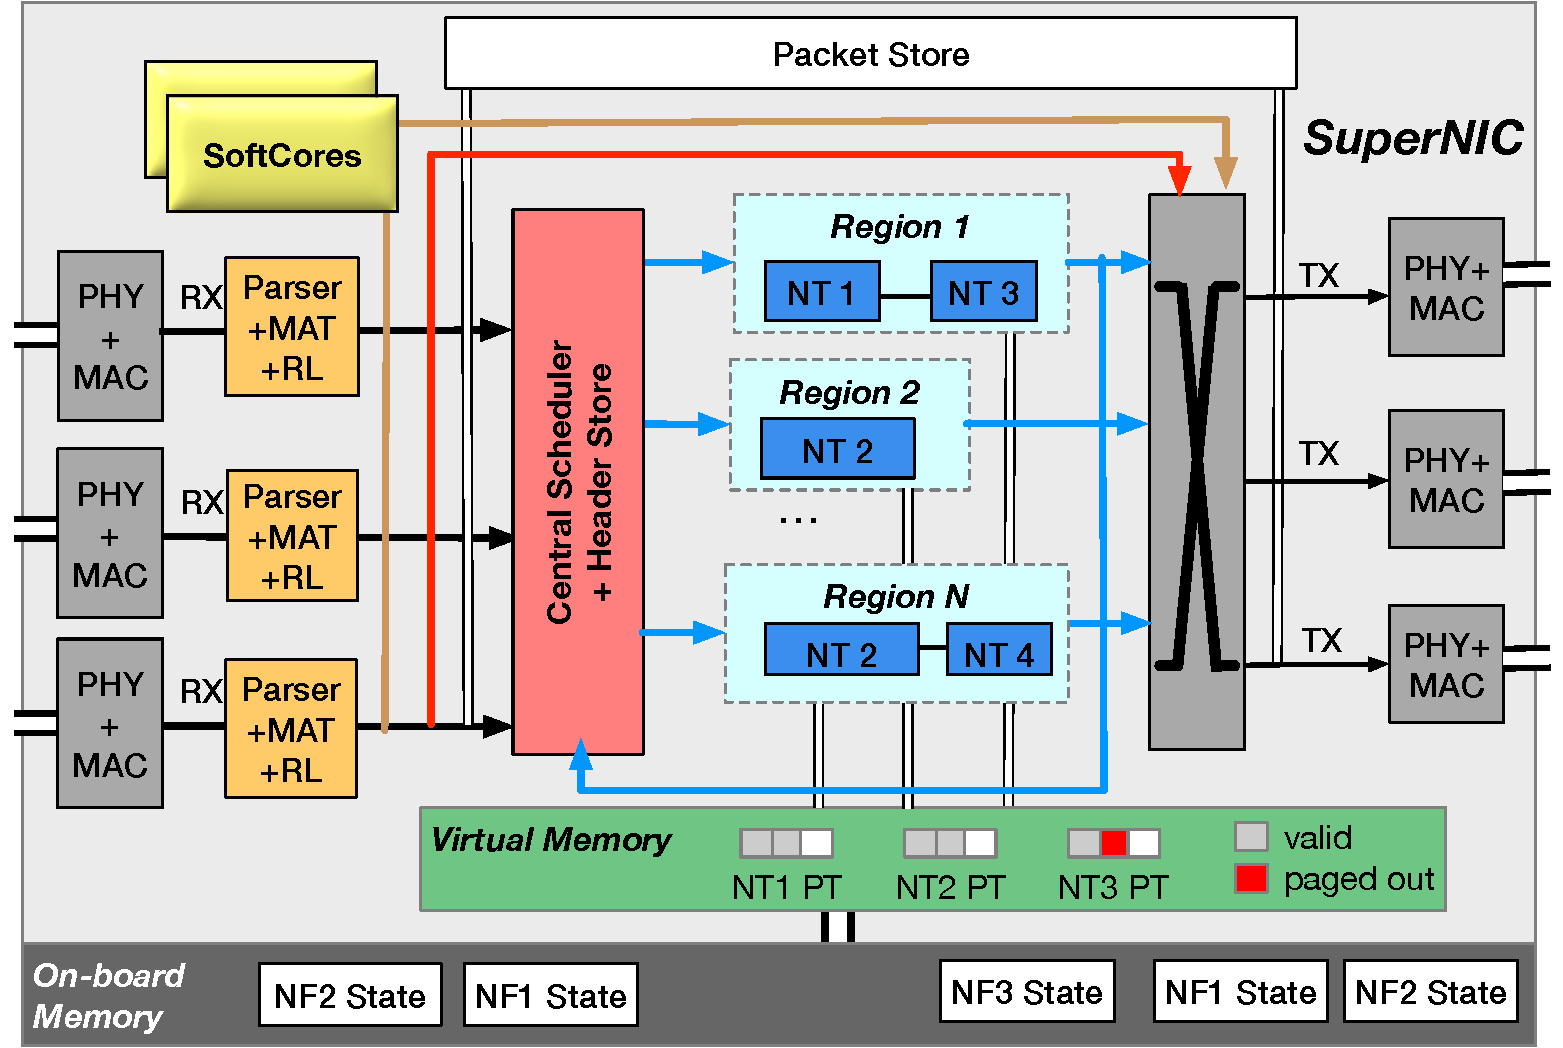
\includegraphics[width=\textwidth]{snic/Figures/board.pdf}}
\mycaption{fig-snic-board}{\snic\ On-Board Design.}
{
RL: Rate Limiter. PT: Page Table
}
\end{center}
\end{figure*}
}
{
\begin{figure*}[th]
\begin{center}
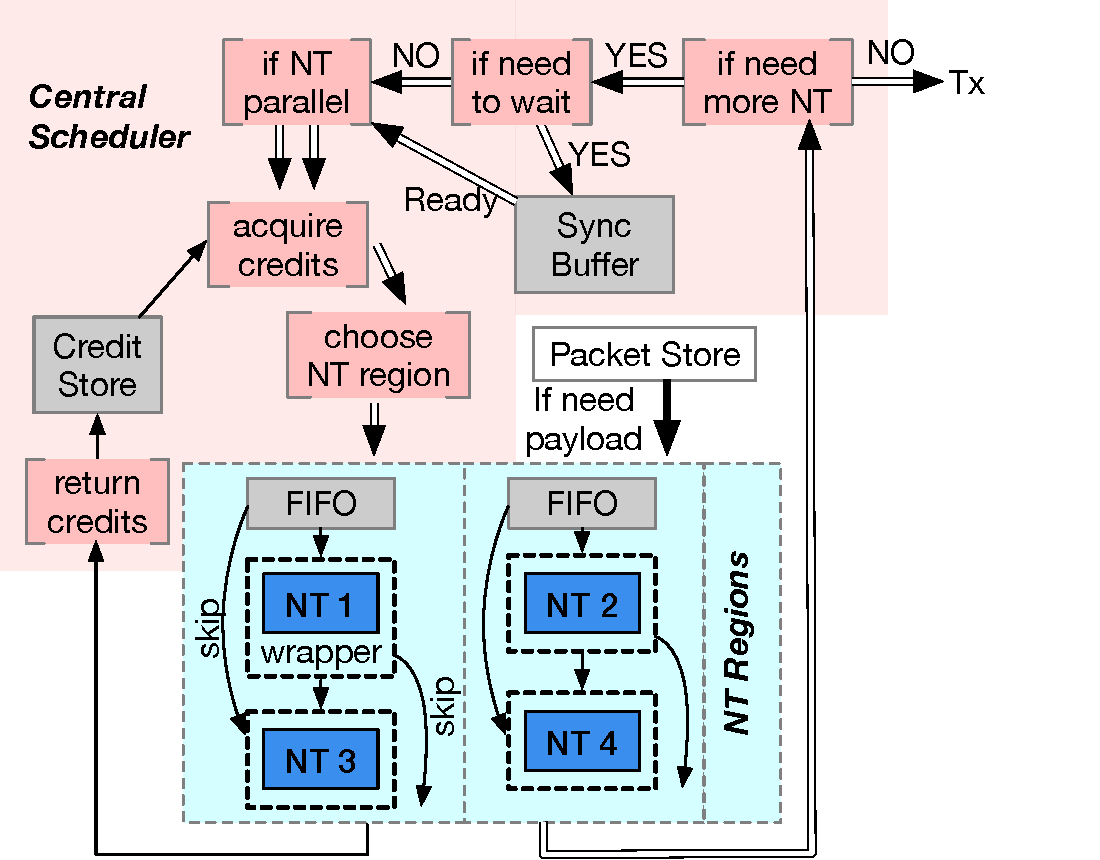
\includegraphics[width=0.9\textwidth]{snic/Figures/scheduler.pdf}
\mycaption{fig-sched}{\snic\ Packet Scheduler and \nt\ Region Design.}
{
Double arrows, single arrows, and thick arrows represent packet headers, credits, and packet payload.
}
\end{center}
\end{figure*}
}

Traditional server SmartNICs have plenty of hardware resources when hosting network functions for applications running on the local server~\cite{SmartNIC-nsdi18,Caulfield-2018}.
In contrast, \snic{} is anticipated to often be fully occupied or even over-committed, as it needs to host \nt{}s from more tenants with limited hardware resources to save costs.
Thus, a key and unique challenge in designing \snic{}s is space- and performance-efficient consolidation in a multi-tenant environment.
Moreover, \snic\ faces a more dynamic environment where not only the load of an application but also applications themselves could change from time to time.
Thus, unlike traditional SmartNICs that focus on packet processing and packet scheduling, \snic\ also needs to schedule \nt{}s efficiently.
%, and both types of scheduling needs to accommodate to a dynamic, multi-tenant environment.
%be more scalable and more flexible.
This section first goes over the high-level architecture of \snic, then discusses our mechanisms for efficient packet and \nt\ scheduling, followed by the discussion of our scheduling and fairness policies, and ends with a description of \snic's virtual memory system.
%We handle the former with SoftCores and the latter with hardware.
%An \snic\ has three major tasks: packet processing, packet scheduling, and \nt\ scheduling.
%overall approach \fixme{TODO if have space}  

\subsection{Board Architecture and Packet Flow}

We design the \snic\ board to simultaneously achieve several critical goals:
\textbf{G1)} parsing/de-parsing and scheduling packets at line rate;
\textbf{G2)} high-throughput, low-latency execution of \nt\ DAGs;
\textbf{G3)} safe and fair sharing of all on-board resources;
\textbf{G4)} quick adaptation to traffic load and workload changes;
\textbf{G5)} good scalability to handle many concurrent workloads and \nt{}s;
\textbf{G6)} flexible configuration and adjustment of control-plane policies;
and \textbf{G7)} efficient usage of on-board hardware resources.
%using most of the on-board hardware resources for application \nt{}s.
Figure~\ref{fig-snic-board} illustrates the high-level architecture of the \snic\ board.

\snic's data plane consists of reconfigurable hardware (\eg, FPGA) for running user \nt{}s (blue parts in Figure~\ref{fig-snic-board})
and a small amount of non-reconfigurable hardware (ASIC) for non-user functionalities, similar to the ``shell'' or ``OS'' concept~\cite{Catapult-v2,Amazon-F1,amorphos-osdi18,coyote-osdi20}.
We choose a hardware-based data-plane design because \nt{}s like transports demand high-speed, parallel processing, and a fully reconfigurable hardware allows the maximum flexibility in \nt\ hardware designs.
Many of our design ideas can potentially be applied to other types of hardware and software \nt\ implementations, such as PISA pipelines and ARM cores.
%In our prototype, 90\% space of the \snic\ chip is dedicated for \nt{}s (\textbf{G7}).

We divide the \nt\ area into {\em region}s, each of which could be individually reprogrammed to run different \nt{}s.
Different \nt\ regions can be executed in parallel.

The control plane runs as software on a small set of general-purpose cores (SoftCores for short) (\eg, a small ARM-based SoC). 
To achieve the performance that the data plane requires and the flexibility that the control plane needs, we cleanly separate these two planes.
The data plane handles all packet processing on ASIC and FPGA (\textbf{G1}).
The control plane is responsible for setting up policies and scheduling \nt{}s and is handled by the SoftCores (\textbf{G6}).
In our prototype, we built everything on FPGA. 


When a packet arrives at an RX port, it goes through a standard physical and reliable link layer.
Then our parser parses the packet's header and uses a Match-and-Action Table (MAT) to decide where to route the packet next.
The parser also performs rate limiting for multi-tenancy fairness (\S\ref{sec:snic:policy}).
The parser creates a packet descriptor for each packet and attaches it to its header. The descriptor contains fields for storing metadata, such as an \nt\ DAG UID and the address of the payload in the packet store. 
The SoftCores determine and install rules in the MAT, which include three cases for routing packets to the next step.
%There are three cases.
First, if a packet specifies no \nt\ information or is supposed to be handled by another \snic\ (\S\ref{sec:snic:dist}), the \snic\ will only perform simple switching functionality and send it to the corresponding TX port (red line).
Second, if a packet specifies the operation type \texttt{CTRL}, it will be routed to the SoftCores (orange line). These packets are for control tasks like adding or removing \nt{}s, adding \nt\ DAGs (\S\ref{sec:snic:ntsched}), and control messages sent from other \snic{}s (\S\ref{sec:snic:dist}).

Finally, all the remaining packets need to be processed on the \snic, which is the common case.
Their payloads are sent to the {\em packet store}, and their headers go to a central scheduler (black arrows). 
The scheduler determines when and which \nt\ chain(s) will serve a packet and sends the packet to the corresponding region(s) for execution (blue arrows).
If an \nt\ needs the payload for processing, the payload is fetched from the packet store and sent to the \nt.
During the execution, an \nt\ could access the on-board memory through a virtual memory interface, in addition to accessing on-chip memory.
After an \nt\ chain finishes, if there are more \nt{}s to be executed, the packet is sent back to the scheduler to begin another round of scheduling and execution.
When all \nt{}s are done, the packet is sent to the corresponding TX port.
%, which uses an arbiter to guarantee bandwidth fairness across applications.


\subsection{Packet Scheduling Mechanism}
\label{sec:snic:packetsched}

We now discuss the design of \snic's packet scheduling mechanism. Figure~\ref{fig-sched} illustrates the overall flow of \snic's packet scheduling and execution.
%To efficiently execute such complex \nt\ DAGs, we first propose the concept of {\em \nt\ chain}, which allows one packet to be processed by a chain of \nt{}s without the need to go through the scheduler multiple times.
%Second, we build a flexible run-time system that supports both {\em \nt-level parallelism} (running different \nt{}s in parallel) and {\em instance-level parallelism} (running multiple instances of the same \nt{}s in parallel) in hardware.
%Existing hardware-based network function systems like Click~\cite{clicknp-sigcomm16}, E2~\cite{e2-sosp15}, and PANIC~\cite{panic-osdi20} focus on scheduling a single NF or a simple sequence of NFs with instance-level parallelism.
%\snic\ provides all three types of scheduling: \nt\ chaining, \nt-level parallelism, and instance-level parallelism, and in a scalable, efficient way.
%Doing so achieves high-throughput, low-latency \nt\ DAG execution (\textbf{G2}), quick adaptation to traffic load changes (\textbf{G4}), and fast and scalable scheduling (\textbf{G5}).

\bolditpara{\nt-chain-based FPGA architecture and scheduling.}
%Today's network systems are seeing increasing amounts of network functions that can be executed as a DAG (\eg, previous work found 53.8\% NF pairs can run in parallel~\cite{NFP-sigcomm17}).
As \snic\ enables more types of endpoints and workloads to offload their network tasks, the number of \nt{}s and their execution flows will become even more complex, which could impact both the complexity of board design and the performance of packet scheduling.
Our idea to confront these challenges is to execute as many \nt{}s as possible in one go, by chaining \nt{}s together.
%There can be different ways to split an \nt\ DAG can 
We put chained \nt{}s (called an {\em \nt\ chain}) in one \nt\ region (\eg, \nt{}1$\xrightarrow[]{}$\nt{}3 and \nt{}2$\xrightarrow[]{}$\nt{}4 in Figure~\ref{fig-snic-board}).
%A packet that uses a chain goes through all the \nt{}s in the chain without the need to involve the scheduler in between.
Instead of connecting each \nt\ to a central scheduler (as what PANIC~\cite{panic-osdi20} does), we connect each region to the scheduler.
Doing so allows us to use a much smaller crossbar between the \nt\ regions and the central scheduler, thereby reducing hardware complexity and area cost (\textbf{G7}).

Furthermore, we leverage \nt\ chains to reduce the scheduling overhead and improve the scalability of the central scheduler.
Our idea is to {\em reserve} credits for an {\em entire} \nt\ chain as much as possible and then execute the chain as a whole; only when that is not possible, we fall back to a mechanism that may involve the scheduler in the middle of a chain. 
Doing so reduces the need for a packet to go through the scheduler after every \nt, thereby improving both the packet's processing latency and the central scheduler's scalability (\textbf{G5}).

On top of the fixed chain design, we propose an optimization to enable efficient \nt\ time sharing across multiple users and to accommodate cases where some packets of an application only access a part of a chain (\textbf{G4}, \textbf{G6}).
Our idea is to support the {\em skipping} of arbitrary \nt(s) in a chain.
For example, a user can access \nt{}1 and \nt{}4 by first skipping \nt{}3 in Region-1 and then skipping \nt{}2 in Region-2 in Figure~\ref{fig-sched}.


\noindent{\ul{\textbf{Scheduling packets with \nt-level and instance-level parallelism.}}}~~
At an \snic, different regions run in parallel.
We exploit two types of parallelism by controlling what \nt{}s to put in parallel regions.
The first type concurrently executes {\em different packets} at multiple instances of the {\em same \nt\ chain} (what we call {\em instance-level parallelism}).
We automatically create more/less instances of an \nt\ chain based on load and send different packets in a round-robin way to the parallel instances.
We will discuss our \nt\ autoscaling policy in \ref{sec:snic:policy}.


The second type concurrently executes the {\em same packet} at multiple {\em different \nt{}s} (what we call {\em \nt-level parallelism}).
We infer what \nt{}s can run in parallel in an \nt\ DAG (\eg, in Figure~\ref{fig-nt-example}, \nt{}1 and \nt{}2 can run in parallel with \nt{}3 for user1).
We expect a fair amount of opportunities to explore \nt-level parallelism, as previous work found that 53.8\% NF pairs can run in parallel~\cite{NFP-sigcomm17}.
To execute a packet at several \nt{}s concurrently, the scheduler makes copies of the packet header and sends them to these \nt{}s concurrently. To obey the order of \nt{}s that users specify, we maintain a {\em synchronization buffer} to store packet headers after they return from an \nt{}'s execution and before they could go to the next stage of \nt{}s (Figure~\ref{fig-sched}).

{
\begin{figure*}
\begin{center}
\centerline{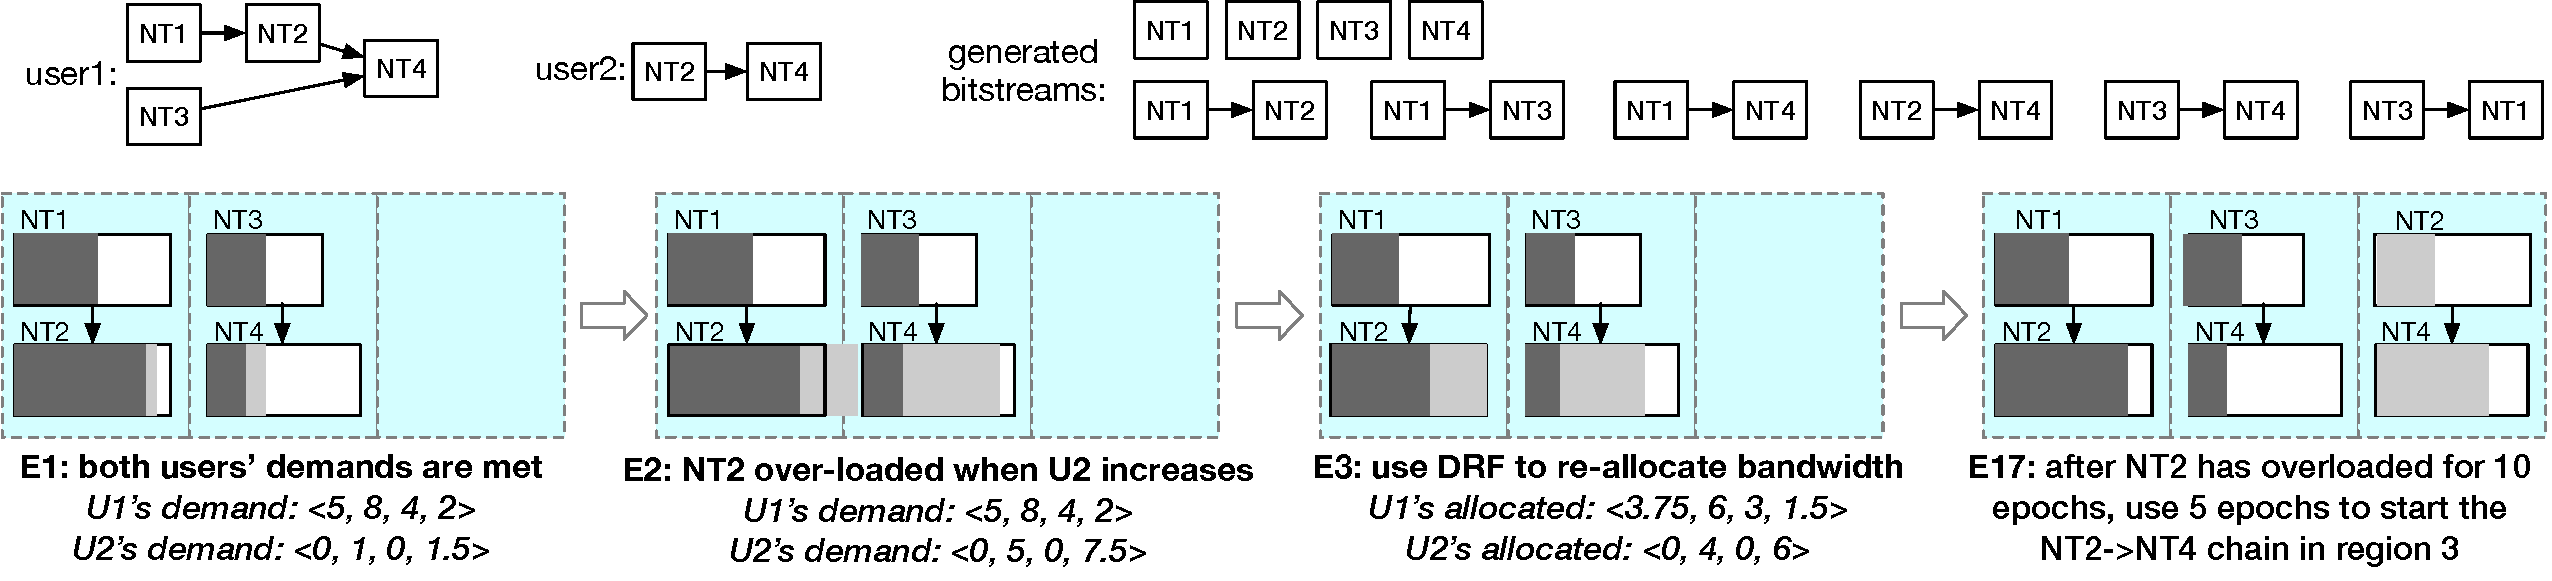
\includegraphics[width=0.9\textwidth]{Figures/nt-example.pdf}}
\vspace{-0.1in}
\mycaption{fig-nt-example}{An Example of \nt\ chaining and scheduling.}
{
Top: user1 and user2's \nt\ DAGs and \snic's generated bitstreams for them.
Bottom: timeline of \nt\ bandwidth allocation change.
Dark grey and light grey represent user1 and user2's load.
The launched chains are \nt{}1$\xrightarrow[]{}$\nt{}2 and \nt{}3$\xrightarrow[]{}$\nt{}4,
with \nt{}2 and \nt{}4 being shared by the two users.
The maximum throughput of NT1, NT2, and NT4 are 10 units each, and NT3's is 7 units.
NT2 is the dominant resource for user1, and NT4 is the dominant for user2.
}
\end{center}
\vspace{-0.2in}
\end{figure*}
}


\subsection{\nt\ (De-)Launching Mechanism}
\label{sec:snic:ntsched}
\snic's SoftCore handles \nt\ deployment, launch, and scheduling tasks, as a part of the control path.
A new challenge specific to \snic\ comes from the need to do more frequent \nt\ reconfigurations than traditional programmable network devices.
To enable more consolidation, we allow multiple \nt{}s to {\em time share} an FPGA space, and we auto-scale \nt{}s.
Both these cases involve the slow FPGA PR process.
We propose a set of new mechanisms and policies to reduce or hide the PR costs.
We now discuss the mechanisms and defer the policy discussions to \S\ref{sec:snic:policy}.

\bolditpara{\nt\ deployment.}~~
Users deploy \nt{}s to the \snic\ platform ahead of time as FPGA netlists (which can be thought of as Intermediate Representations in software).
When receiving newly deployed \nt{} netlists for an application, we first generate a set of FPGA bitstreams (which can be thought of as executable binaries in software).
We enumerate all possible combinations of \nt{}s under user-specified \nt\ DAG ordering requirements when generating bitstreams. 
This is because bitstream generation is a slow process that usually takes a few hours or even longer. 
Generating more bitstreams at deployment time gives the \snic\ more flexibility to choose different \nt\ combinations at the run time. 
Figure~\ref{fig-nt-example} shows an example of generated bitstreams based on two DAGs of two users.
%\noteyiying{delete the following sentence if need more space}
%We do not generate bitstreams for three-\nt{} chains in this example, as that exceeds what a region can hold.
%For example, with three \nt{}s where the user specifies the first two to fan in to the third, we generate bitstreams for \nt{}1, \nt{}2, \nt{}3, \nt{}1$\xrightarrow{}$\nt{}2, \nt{}2$\xrightarrow{}$\nt{}1, \nt{}1$\xrightarrow{}$\nt{}3, \nt{}2$\xrightarrow{}$\nt{}3, \nt{}1$\xrightarrow{}$\nt{}2$\xrightarrow{}$\nt{}3, and \nt{}2$\xrightarrow{}$\nt{}1$\xrightarrow{}$\nt{}3.
We store pre-generated bitstreams in the \snic{}'s on-board memory; each bitstream is small, normally less than 5\MB.

When generating bitstreams, we attach a small \snic\ wrapper to each \nt\ (Figure~\ref{fig-sched}).
%This module monitors the load of each \nt\ and \yiying{Will, what else is in the module?}
This wrapper is essential: it enables skipping an \nt\ in a chain (\S\ref{sec:snic:packetsched}), monitors the runtime load of the \nt\ (\S\ref{sec:snic:policy}), ensures signal integrity during PR, and provides a set of virtual interfaces for \nt{}s to access other board resources like on-board memory (\S\ref{sec:snic:memory}).

\bolditpara{\nt\ chain launching.}~~
We start a new \nt\ chain when an application is deployed (pre-launch), when the chain is first accessed by a packet in an application (on-demand), or when we scale out an existing \nt\ chain. For the first and third cases, we start the new \nt\ only when there is a free region (see \S\ref{sec:snic:policy} for detail).
%The SoftCore picks a free region to launch the chain. 
For the on-demand launching case, when all regions are full, we still need to launch the new chain to be able to serve the application. In this case, we need to de-schedule a current \nt\ chain to launch the new chain (see \S\ref{sec:snic:policy} for how we pick the region).

The \snic\ SoftCore handles this context switching with a {\em stop-and-launch} process.
Specifically, the SoftCore sends a signal to the current \nt{}s to let them ``stop''.
These \nt{}s then store their states in on-board memory to prepare for the stop.
At the same time, the SoftCore informs the scheduler to stop accepting new packets. 
The scheduler will buffer packets received after this point.
After the above {\em stop step}s finish, the SoftCore reads the new bitstream from the on-board memory via DMA and starts the FPGA PR process ({\em launch}).
This process is the slowest step, as the maximum reported achievable PR throughput is around 800\,MB/s~\cite{coyote-osdi20}, or about 5\,\ms\ for our default region size.
Afterwards, the newly launched chain can start serving packets, and it will first serve previously buffered packets, if any.

%\boldpara{Swap and victim region.}~~
%A unique and new challenge in scheduling \nt{}s in FPGA is that unlike software, the \nt\ region reconfiguration process as described above is slow. 
%We tackle this challenge from both the mechanism and policy perspectives.
%We now discuss our ideas in mechanisms.

To reduce the overhead caused by \nt\ reconfiguration, we use a technique similar to the traditional victim cache design. We keep a de-scheduled \nt\ chain in a region around for a while unless the region is needed to launch a new chain. If the de-scheduled \nt\ chain is accessed again during this time, we can directly use it in that region, reducing the need to do PR at that time.

%we always leave one or few regions empty; we call them {\em swap region}s.
%To start a new chain, the SoftCore directly launches it in one swap region and start processing new packets with it.
%In the background, the SoftCore de-schedule an \nt\ chain by performing the {\em stop} step as illustrated above to create one more swap region.
%This swap region approach allows us to reduce the reconfiguration time to only the {\em launch} time. 

%Our second idea is inspired by victim cache in the traditional CPU architecture. 
%When de-scheduling an \nt\ chain, instead of clear the region, we leave it as is and tag it as a special {\em victim swap region}.
%If a swap region is needed to launch a new chain, this region can be picked.
%Otherwise, before it's picked, if packets access this chain again, they can directly use the region.
%If the chain's load is increased to be more than another chain's load, this other chain's region will be marked as the victim region, and the original victim region becomes a normal region.
%Our victim region approach avoids the overhead of de-scheduling and launching an \nt\ chain when there's only a short period of low load.

\subsection{Packet and \nt\ Scheduling Policy}
\label{sec:snic:policy}

We now discuss our packet and \nt\ scheduling policies.
Figure~\ref{fig-nt-example} shows an example of how an \snic\ with three regions evolves as load changes.

\bolditpara{Overall \nt\ scheduling strategy.}~~
Our overall strategy is to avoid FPGA PR as much as possible and treat \nt\ context switching (\ie, replacing a current \nt\ chain with a new one through FPGA PR) as a last resort, since context switching prevents the old \nt\ from running altogether and could result in thrashing in the worst case. 

For on-demand \nt\ launching, we first check if the \nt\ is the same as any existing \nt{} on the \snic.
If so, and if the existing \nt{} still has available bandwidth, we time share the existing \nt\ with the new application. %(\circled{1}).
In this case, new traffic can be served immediately.
Otherwise, we check if there is a free region.
If so, we launch the \nt\ at this region, and new traffic can be served after FPGA PR finishes.
Otherwise, we reach out to the distributed \snic\ platform and check if any other \snic\ has the same \nt\ with available bandwidth or a free region. 
If so, we route traffic to that \snic\ (to be discussed in \S\ref{sec:snic:dist}).
Otherwise, we run the \nt\ at the endpoint if users provide the alternative way of executing it there.
%user an alternative way of launching the \nt, \eg, running in hardware or software at the endpoint.
If all of the above fail, we resort to context switching by picking the region that is least loaded and using stop-and-launch to start the \nt.

We also try to hide PR latency behind the performance-critical path as much as possible.
%This is because it is slow to switch contexts (involving reconfiguring \nt{}s) and the 
Specifically, when a new application is deployed, we check if any of its \nt{}s is missing on an \snic. If there are any and if there are free regions on the \snic\ for these \nt{}s, we {\em pre-launch} them at the free regions, instead of launching them {\em on-demand} when the first packet accesses the \nt{}s, as the latter would require waiting for the slow PR and slow down the first few packets. 
%These pre-launched \nt{}s are the first batch of victims we choose to de-schedule if free regions are needed for other \nt{}s.

\bolditpara{\nt\ auto-scaling.}~~
To adapt to load changes, \snic\ automatically scales out/down instances of the same \nt\ (instance-level parallelism) (\textbf{G2, G4}).
Specifically, we use our per-\nt\ monitoring module to identify bottleneck \nt{}s and the load that they are expected to handle.
If there are free regions, we add more instances of these \nt{}s by performing PR on the free regions.
When the load to an \nt\ reduces to what can be handled with one instance less, we stop one of its instances and migrate the traffic of the stopped instance to other running instances.
Since PR is slow, we should scale out/down an \nt\ only if there is a persistent load increase/decrease instead of just occasional load spikes.
To do so, we only scale out/down an \nt\ if the past \texttt{MONITOR\_PERIOD} time has overloaded/underloaded the \nt.
\texttt{MONITOR\_PERIOD} should be at least longer than the PR latency to avoid thrashing. Since our measured PR latency is 5\ms, we set \texttt{MONITOR\_PERIOD} to be 5\ms\ by default. 
After experimenting other length, we find this length to work the best with most real-world traffic~\cite{facebook-sigcomm15,Atikoglu12-SIGMETRICS}.
%\noteyiying{Update this after getting Will's new monitoring sensitivity results.}
%\texttt{HIGH\_LOAD} is a heuristic depending on workloads.
%Previous works have reported different traffic peak lengths~\cite{facebook-sigcomm15,facebook-sigmetrics12}, \eg, millisecond-level in the 2015 Facebook trace~\cite{facebook-sigcomm15}, for which we could set \texttt{HIGH\_LOAD} to \fixme{XXX}.

\bolditpara{Scheduling with fairness.}~~
As we target a multi-tenant environment, \snic\ needs to fairly allocate its resources to different applications (\textbf{G3}).
%On top of the above strategy, we seek fairness across applications.
Different from existing fairness solutions, we treat every \nt\ as a separate type of resource, in addition to ingress bandwidth, egress bandwidth, packet store, and on-board memory space.
This is because we support the time sharing of an \nt, and different \nt{}s can be shared by different sets of users. Our fairness policy follows Dominant Resource Fairness (DRF)~\cite{DRF}, where we identify the {\em dominant} resource type for each application and seek a fair share for each application's dominant type. We also support weighted DRF~\cite{DRF,beyond-DRF} for users with different priorities.

Instead of a user-supplied static resource demand vector used in traditional DRF systems, we use {\em dynamically monitored resource demands} as the target in the DRF algorithm.
Specifically, at each {\em epoch}, we use the ingress parser, egress de-parser, the central scheduler, and our virtual memory system to monitor the actual load demand before requests are dispatched to a particular type of resource.
For example, for each user, the central scheduler measures the rate of packets that should be sent next to an \nt\ before assigning credits; \ie, even if there is no credit for the \nt, we still capture the intended load it should handle.
Based on the measured load at every type of resource for an application, we determine the dominant type of resource and use DRF to allocate resources after considering all applications' measured load vectors.
At the end of every epoch, our DRF algorithm outputs a new vector of resource allocation for each application, which the next epoch will use.
Compared to static resource demand vectors, our run-time monitoring and dynamic resource vectors can promptly adapt to load changes to maximize resource utilization. % with a higher degree of consolidation.

%We rerun the DRF algorithm right after scaling out/down an \nt{}, since scaling essentially changes the ``cap'' of the \nt's resource amount.

Another novelty is in how we achieve the assigned allocation.
Instead of throttling an application's packets at each \nt\ and every type of resource to match the DRF allocation, we only control the application's ingress bandwidth allocation.
Our observation is that since each \nt's throughput for an application, its packet buffer space consumption, and egress bandwidth are all proportional to its ingress bandwidth, we could effectively control these allocations through the ingress bandwidth allocation.
Doing so avoids the complexity of throttling management at every type of resource.
Moreover, throttling traffic early on at the ingress ports helps reduce the load going to the central scheduler and the amount of payload going to the packet store.
Our current implementation controls ingress bandwidth through rate limiting.
Future work could also use other mechanisms like Weighted Fair Queuing.
The only resource that is not proportional to ingress bandwidth is on-board memory space.
We control it through our virtual memory system (\S\ref{sec:snic:memory}).

Finally, the length of an epoch, \texttt{EPOCH\_LEN}, is a configurable parameter.
At every epoch, we need to run the DRF algorithm and possibly change the bandwidth and memory allocation.
Thus, \texttt{EPOCH\_LEN} should be longer than the time taken to perform these operations (around 3\mus\ with our implementation).
%Our measured time is 3\mus\ for running the DRF algorithm, negligible for changing bandwidth, and 15-20\mus\ for swapping out a 2\MB\ page.
%Note that swapping out memory can be done in a lazy fashion and does not complete in an epoch.
Meanwhile, it is desirable to set a short \texttt{EPOCH\_LEN} to quickly adapt to load variations and to update rate allocations approximately once per average RTT~\cite{xcp-sigcomm02, rcp-sigcomm06}.
Thus, we set the default value of \texttt{EPOCH\_LEN} to 20\mus.

\subsection{Virtual Memory System}
\label{sec:snic:memory}
\snic's allow \nt{}s to use off-chip, on-board memory.
To isolate different applications' memory spaces and to allow the over-subscription of physical memory space in an \snic, we build a simple page-based virtual memory system.
\nt{}s access on-board memory via a virtual memory interface,
where each \nt\ has its own virtual address space.
Our virtual memory system translates virtual memory addresses into physical ones and checks access permissions with a single-level page table.
We use huge pages (2\MB\ size) to reduce the amount of on-chip memory to store the page table.
Physical pages are allocated on demand; when a virtual page is first accessed, \snic\ allocates a physical page from a free list.

We further support the over-subscription of an \snic's on-board memory, \ie, an \snic\ can allocate more virtual memory space than its physical memory space.
When the physical memory is full, adding more \nt\ would require shrinking memory already assigned to existing applications (\S\ref{sec:snic:ntsched}).
In this case, we reduce already assigned memory spaces by migrating memory pages to a remote \snic, \ie, swapping out pages.
To decide what pages to swap out, we first use the DRF algorithm to identify what \nt{}(s) should shrink their memory space. 
Within such an \nt, we pick the least recently accessed physical page to swap out.
Our virtual memory system tracks virtual memory accesses to capture per-page access frequency. 
It also transparently swaps in a page when it is accessed.
If no other \snic{} has free memory space when the \snic\ needs to grow its virtual memory space, we reject requests to add new \nt{}s or to enlarge existing \nt{}'s memory.